\subsection{Experimental Implementation Details}
\label{appendix:setups}
We provide a comprehensive list of hyperparameters and implementation details used in our experiments to ensure full reproducibility.

\paragraph{General Setup.}
Across all experiments, we use models from the Qwen2.5 family~\citep{qwen2025qwen25technicalreport} with their corresponding tokenizers. The maximum sequence length is set to 8192 tokens for all inputs, and the maximum response sequence length is set to 1024 tokens. The GPT-4o-mini model is used as the teacher model in the corresponding ablation study. We use BGE-M3~\citep{chen2024bge} as our embedding model.

\paragraph{Cold-start Stage.}
This initial SFT stage is designed solely to teach the model the required interaction format(e.g., producing well-structured \thinktag{think} and \searchtag{search} actions). The model is trained for 3 epochs using the Adam optimizer, with an initial learning rate of $1\times10^{-4}$, a warm-up ratio of 0.1, and a batch size of 16.
% This SFT stage is conducted for 3 epochs using the Adam optimizer, with an initial learning rate of $1\times10^{-4}$, a warm-up ratio of 0.1, and a batch size of 16.

\paragraph{Online Interaction Phase.}
For each \knowledgetag{search\_knowledge} action, we retrieve the top-$k_d=3$ documents from the external knowledge base, following the prior work~\citep{jin2025searchr1trainingllmsreason}. Similarly, for each \searchtag{search\_experience} action, we retrieve the top-$k_e=3$ principles from the experience base $\mathcal{E}$.

\paragraph{Offline Distill Phase.}
The self-distill mechanism utilizes the agent's own policy model $\pi_\theta$ to distill principles. The temperature is set to 1 during this phase. For the deduplication and integration process, we first use a semantic similarity pre-filter with a threshold of $\theta_{\text{sim}} = 0.85$ before passing candidates to the LLM-based equivalence check. The periodic principle sweep removes any principle from $\mathcal{E}$ whose \texttt{metric\_score} falls below the pruning threshold of $\theta_{\text{prune}} = 0.3$.

\paragraph{Reward Function Details.}
As described in the Section~\ref{subsec:policy_evolution}, the Format Reward is an average of a think score and a search score. We detail their specific calculation here. The think score $R_{\text{think}}$ is determined by a discrete mapping based on the number of \thinktag{think} actions, $N_{\text{think}}$: it scales from 0.2 (for $N_{\text{think}}=1$) to a maximum of 1.0 (for $N_{\text{think}}=6$), and is capped at 0.5 for excessive reasoning ($N_{\text{think}}>8$) to encourage conciseness. The search score $R_{\text{search}}$ is the sum of a diversity score and a quantity bonus. The diversity score is 0.5 if both \searchtag{search\_experience} and \knowledgetag{search\_knowledge} are used, 0.2 if only one type is used, and 0 otherwise. A quantity bonus of 0.1 is added for each additional search action beyond the first, up to a maximum bonus of 0.5 (for a total of 6 searches).


\paragraph{Policy Optimization.}
The composite reward function is weighted with $w_o = 1.0$ for the outcome reward and $w_f = 0.1$ for the format reward. For the GRPO objective function (Equation~\ref{eq:grpo_objective}), the clipping parameter is set to $\epsilon = 0.2$ and the KL-divergence coefficient is $\beta = 0.001$. During the training procedure, we adopt vLLM to accelerate LLM rollouts. The tensor
parallel size is set to 1, and the GPU memory utilization ratio is set at 0.6. For rollout sampling, we use a temperature of 1.0 and a top-p value of 0.95.


\paragraph{Computational Cost Analysis.}
We provide detailed computational resources required for training and experience retrieval latency to demonstrate the efficiency of EvolveR.

\begin{itemize}[leftmargin=2em]
    \item \textbf{Training Cost:} The full training lifecycle for the Qwen2.5-3B model, which includes the cold-start SFT phase and the subsequent RL policy evolution via GRPO, requires approximately \textbf{39.4 hours} on a server equipped with 8 NVIDIA A100 (80GB) GPUs. 
    
    \item \textbf{Experience Retrieval Latency:} A key concern for retrieval-augmented systems is the added latency during inference. We implement the Experience Base using Milvus for efficient vector similarity search. Our empirical measurements show that even with an experience base containing approximately \textbf{14,000 principles}, the latency for retrieving the top-3 relevant principles is approximately \textbf{0.06 seconds}. That is imperceptible compared to LLM generation time, ensuring that EvolveR maintains high throughput during deployment.
\end{itemize}



\paragraph{SFT-only Baseline Details.}
We used the exact same set of successful trajectories generated during the Online Interaction stage. Both \exptag{experience} and \infotag{information} tokens were masked during training. We utilised the LLaMAFactory~\cite{zheng2024llamafactory} to fine-tune the Qwen2.5-3B model using LoRA (Low-Rank Adaptation). The LoRA rank is set to 8, the learning rate is $1\times10^{-4}$, and the model is trained for 5 epochs with a batch size of 1. The warmup ratio is 0.1, the maximum sequence length is 4096 tokens, gradient accumulation steps are set to 8, and the learning rate scheduler is \texttt{Cosine}.

\subsection{Additional Experimental Analysis}
\label{sec:additional_exp_analysis}

\subsubsection{Necessity of the RL (GRPO) Stage}
% In this setting, we replace GRPO with a supervised fine-tuning (SFT) variant.

To assess the necessity of the Reinforcement Learning stage in \texttt{EvolveR}, we conduct an ablation experiment on the Qwen2.5-3B model. Specifically, we reuse the exact same set of successful trajectories collected during online interaction, but train the policy via standard SFT rather than GRPO. The full SFT hyperparameter configurations are provided in Section~\ref{appendix:setups}.


As shown in Table~\ref{tab:ablation_sft}, the RL-based variant substantially outperforms the SFT-only version on the 3B model, achieving a 7\% relative improvement. This result highlights the fundamental limitation of SFT: it merely encourages the model to reproduce surface-level action sequences from successful trajectories, without understanding the underlying utility or expected reward of actions such as \searchtag{search\_experience}. In contrast, our RL approach (GRPO) leverages both successful and failed trajectories, enabling the agent to learn \emph{what to do} from positive rollouts and \emph{what to avoid} from negative ones, which is essential for developing robust retrieval and reasoning strategies.



\begin{table*}[!ht]
    \centering
    \small
    \setlength{\tabcolsep}{4pt}
    \vspace{-1em}
    \caption{Comparison between SFT-only and RL/GRPO training in EvolveR on the Qwen2.5-3B model.}
    \label{tab:ablation_sft}
    \begin{tabular}{l cc ccccc c}
        \toprule
        \multirow{2}{*}{\textbf{Model Variant}}  & \multicolumn{2}{c}{\textbf{In domain}} & \multicolumn{5}{c}{\textbf{Out of domain}} & \multirow{2}{*}{\textbf{Avg.}} \\
        \cmidrule(lr){2-3} \cmidrule(lr){4-8}
        & NQ \phup & HotpotQA \phup & TriviaQA \phup & PopQA \phup & 2wiki \phup & Musique \phup & Bamboogle \phup & \\
        \midrule
        EvolveR(SFT)& 0.415& 0.357& 0.584& 0.419& 0.366& 0.106& 0.248& 0.357\\
        EvolveR(RL)& \textbf{0.434} & \textbf{0.373} & \textbf{0.584} & \textbf{0.434} & \textbf{0.381} & \textbf{0.137} & \textbf{0.328} & \textbf{0.382} \\
        \midrule
    \end{tabular}
\end{table*}

\subsubsection{Hyperparameter Sensitivity Analysis}
\label{sec:sensitivity_analysis}
To assess the robustness of EvolveR and the impact of the dynamic experience curation mechanism, we conducted a sensitivity analysis on the pruning threshold $\theta_{\text{prune}}$, the results are provided in the Table~\ref{tab:sensitivity_prune}. This parameter dictates the minimum \texttt{metric\_score} required for a principle to be retained in the Experience Base after each cleaning. We evaluated the performance of the EvolveR-1.5B model across a wide range of thresholds: $\theta_{\text{prune}} \in \{0.1, 0.3, 0.7, 0.9\}$.

\begin{table*}[!ht]
    \centering
    \small
    \setlength{\tabcolsep}{4pt}
    \vspace{-1em}
    \caption{Sensitivity analysis of the pruning threshold $\theta_{\text{prune}}$ on the Qwen2.5-1.5B model.}
    \label{tab:sensitivity_prune}
    \begin{tabular}{l cc ccccc c}
        \toprule
        \multirow{2}{*}{\textbf{$\theta_{\text{prune}}$}} & \multicolumn{2}{c}{\textbf{In domain}} & \multicolumn{5}{c}{\textbf{Out of domain}} & \multirow{2}{*}{\textbf{Avg.}} \\
        \cmidrule(lr){2-3} \cmidrule(lr){4-8}
        & NQ \phup & HotpotQA \phup & TriviaQA \phup & PopQA \phup & 2wiki \phup & Musique \phup & Bamboogle \phup & \\
        \midrule
        0.1 (loose) & 0.336 & 0.244 & 0.496 & 0.387 & \textbf{0.207} & 0.052 & 0.160 & 0.269 \\
        0.3 (Default) & \textbf{0.358} & \textbf{0.257} & \textbf{0.510} & \textbf{0.389} & 0.188 & 0.057 & 0.128 & 0.270 \\
        0.7 (strict) & 0.276 & 0.253 & 0.498 & 0.379 & 0.196 & 0.060 & \textbf{0.192} & 0.265 \\
        0.9 (very strict) & 0.323 & \textbf{0.257} & \textbf{0.510} & 0.385 & 0.204 & \textbf{0.061} & \textbf{0.192} & \textbf{0.276} \\
        \bottomrule
    \end{tabular}
\end{table*}

The results confirm that performance remains robust across different thresholds. Our default setting ($\theta_{prune}=0.3$) effectively filters out low-quality principles to prevent the database from growing indefinitely. 




\subsubsection{Longitudinal Analysis of Learning Dynamics}
\label{sec:longitudinal_analysis}

To provide a deeper understanding of how the EvolveR agent improves over time, we present a longitudinal analysis of its behavior during the RL training process. We focus on two key aspects: the evolution of action frequencies and the improvement in the quality of distilled principles.

\paragraph{Evolution of Action Frequencies.}
We tracked the average number of \texttt{<think>}, \texttt{<search\_knowledge>} and \texttt{<search\_experience>} actions per trajectory across training steps. As shown in Figure~\ref{fig:action_evolution}, the agent's behavior exhibits distinct phases of optimization:

\begin{itemize}[leftmargin=2em]
    \item \textbf{Early Phase (Interval 1):} Thanks to the cold-start SFT, the agent begins with reasonable tool usage capabilities.
    \item \textbf{Optimization Phase (Intervals 2-3):} As RL training progresses, we observe a clear upward trend in the frequency of \texttt{<think>} and \texttt{<search\_knowledge>}. This indicates that the agent is learning to engage in deeper reasoning and more extensive external information gathering to solve complex tasks.
    \item \textbf{Convergence Phase (Interval 4):} Crucially, the action counts do not increase indefinitely. They converge to a stable, efficient range (approx. 2 experience searches, 4 knowledge searches, and 6 reasoning steps).
\end{itemize}

\begin{figure}[h]
    \centering
    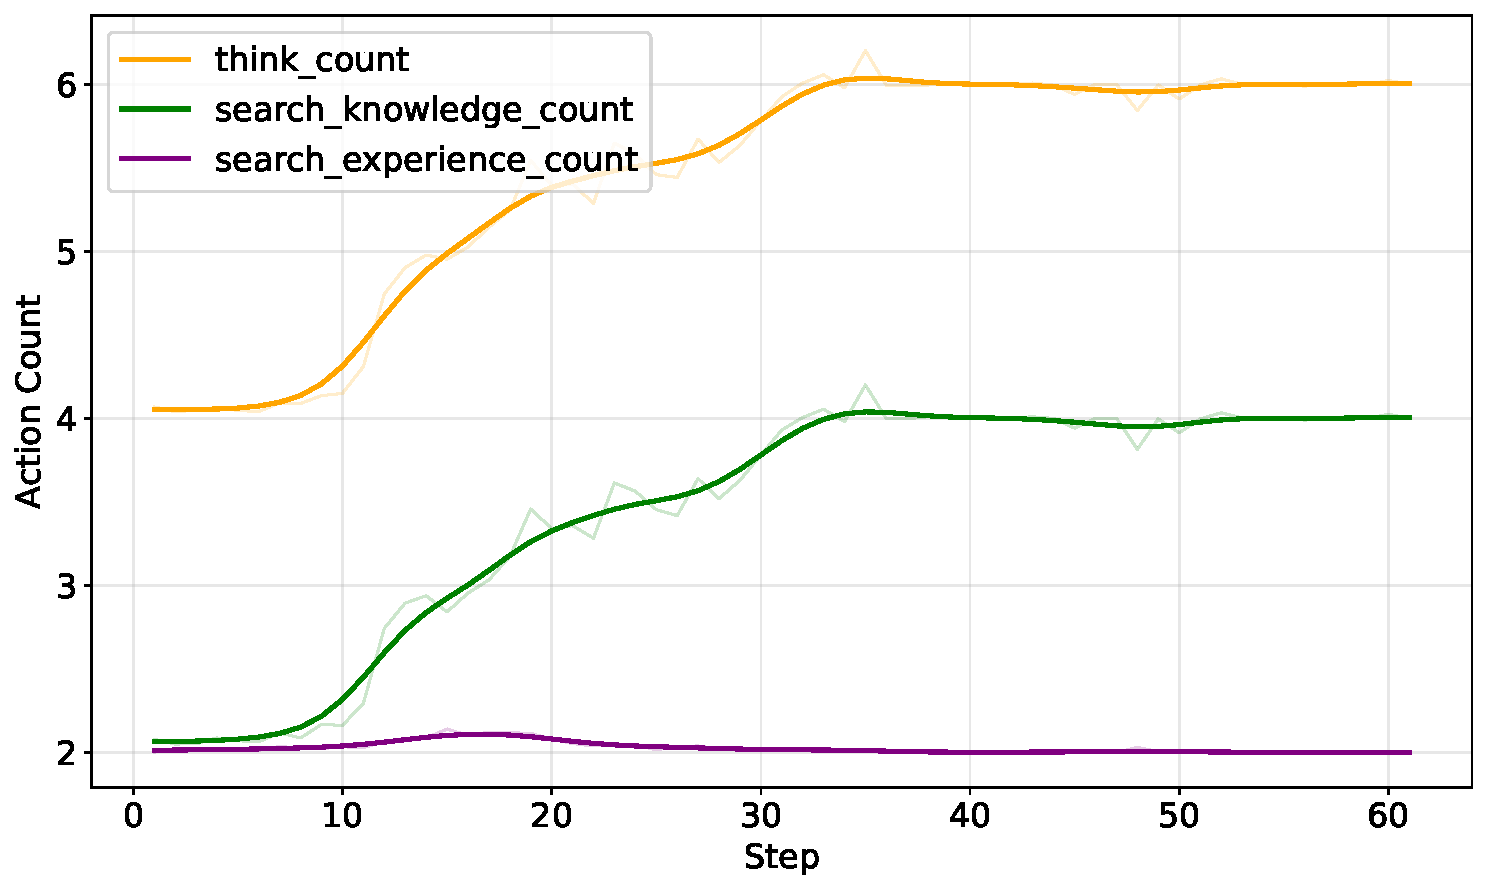
\includegraphics[width=1\linewidth]{img/action_counts_curve-step_61.pdf}
    \caption{Evolution of average action counts per trajectory during RL training.}
    \label{fig:action_evolution}
\end{figure}


\paragraph{Intrinsic Improvement in Principle Distillation.}
To verify that the agent is indeed improving its ability to distill high-quality principles (rather than just filtering out bad ones), we analyzed the quality of principles grouped by their distilled time. We divided the training process into four intervals and calculated the average \texttt{metric\_score} of the principles generated in each interval that remain in the Experience Base.

\begin{table}[h]
    \centering
    \small
    \caption{Quality of principles by creation phase.}
    \label{tab:principle_quality_evolution}
    \begin{tabular}{lccc}
        \toprule
        \textbf{Creation Phase} & \textbf{Avg. Metric Score} & \textbf{Avg. Usage Count} \\
        \midrule
        Interval 1 & 0.462 & 8.22 \\
        Interval 2 & 0.464 & 24.10 \\
        Interval 3 & 0.487 & 17.82 \\
        Interval 4 & \textbf{0.500} & 12.36\\
        \bottomrule
    \end{tabular}
\end{table}

Table~\ref{tab:principle_quality_evolution} presents the evolution of principle quality across different training stages. Principles from Interval 1 have undergone the longest duration of dynamic pruning, representing a highly filtered subset. Conversely, principles from Interval 4 are relatively new and have been subject to less filtering. We observe that the principles generated in the final stage achieve a higher average metric score (0.500) compared to those from the earliest stage (0.462). Supported by substantial usage counts ($>12$) that ensure statistical stability, this trend indicates that the agent's intrinsic ability to distill high-quality strategies improves over time.

\subsection{Exploring the Influence of Experience Internalization}

In our proposed framework, all retrieved information (both from the external knowledge base (\infotag{information}) and our internal experience base (\exptag{experience})) is treated as context, with loss masked during the model update phase. A natural question arises from this design: while it is sensible to avoid learning the content of transient external documents, could the agent benefit from directly `absorbing` its own distilled wisdom into its parameters?

To explore this, we conducted a supplementary experiment on the Qwen2.5-3B model. We created a variant, \texttt{EvolveR w/ exp-absorb}, where we selectively unmasked the loss for the retrieved \exptag{experience} tokens, allowing the learning signal to flow through them. Our hypothesis was that this might enable the agent to internalize the strategic logic of its principles. The results, presented in Table~\ref{tab:ablation_internalization}, were insightful. The \texttt{EvolveR w/ exp-absorb} variant exhibited a slight performance degradation compared to our standard approach. We posit that this is due to the challenge of noise in the training signal. In our current implementation, the agent retrieves a set of top-$k$ principles at each step. Not all of these principles may be perfectly relevant to the immediate context. By directly internalizing all retrieved principles without a dynamic quality filter, the agent risks being updated with noisy or even counter-productive signals. This finding suggests that for direct internalization to be effective, it may require more sophisticated mechanisms, such as an auxiliary model to weigh the relevance of each principle before absorption. We believe that developing such mechanisms is a promising future direction towards achieving a fully autonomous cycle of self-exploration, self-distillation, and self-absorption.

\begin{table*}[!ht]
    \centering
    \small
    \setlength{\tabcolsep}{1.5pt}
    \caption{Ablation study on the experience internalization mechanism. EvolveR w/o exp-absorb treats principles as external context by masking gradients during backpropagation.}
    \label{tab:ablation_internalization}
    \begin{tabular}{l cc ccccc c}
        \toprule
        \multirow{2}{*}{\textbf{Model Variant}} & \multicolumn{2}{c}{\textbf{In domain}} & \multicolumn{5}{c}{\textbf{Out of domain}} & \multirow{2}{*}{\textbf{Avg.}} \\
        \cmidrule(lr){2-3} \cmidrule(lr){4-8}
        & NQ \phup & HotpotQA \phup & TriviaQA \phup & PopQA \phup & 2wiki \phup & Musique \phup & Bamboogle \phup & \\
        \midrule
        EvolveR & 0.434 \phdown & 0.373 \phdown & 0.584 \phdown & 0.434 \phup & 0.381 \phdown & 0.137 \phdown & 0.328 \phdown & 0.382 \phdown \\
        EvolveR w exp-absorb & 0.433 \down & 0.369 \down & 0.583 \down & 0.435 \up & 0.376 \down & 0.124 \down & 0.280 \down & 0.371 \down \\
        \bottomrule
    \end{tabular}
\end{table*}








\subsection{Prompt Details}
\subsubsection{Cold Start Prompt}
The Prompt in Table~\ref{tab:cold_start_prompt} is used during the cold-start stage to generate the initial trajectories for SFT. This prompt guides a powerful LLM (we used GPT-4o) to act as an expert problem-solver, producing a small dataset with right format trajectories to cold start.




\subsubsection{System Prompt}
The Prompt in Table~\ref{tab:system_prompt} is the system prompt used by the EvolveR agent during the online interaction phase. It defines the agent's core identity, its available actions (\thinktag{think}, \knowledgetag{search\_knowledge}, \searchtag{search\_experience}, \answertag{answer}), and the overall format for its reasoning process.



\subsubsection{Distill Principle Prompt}
The Prompt in Table~\ref{tab:success_distill_prompt} and Table~\ref{tab:fail_distill_prompt} are used during the offline experience self-distillation phase to enable the agent's self-distillation mechanism. Based on the outcome of a trajectory, one of two distinct prompts is used to guide the agent's own model ($\pi_\theta$) to distill a principle. The first Prompt is for successful trajectories, focusing on extracting a guiding principle. The second is for failed trajectories, aimed at formulating a cautionary principle.


\subsubsection{Judge Same Principle Prompt}
The Prompt in Table~\ref{tab:match_principle_prompt} is a crucial component of the deduplication and integration process within the offline experience self-distillation. It tasks the agent's own model ($\pi_\theta$) with acting as a semantic judge. Given two principles (a newly distilled candidate and a retrieved existing similar one), the model is asked to determine if they are semantically equivalent. The binary "yes/no" output of this Prompt is used to decide whether to merge a new experience or create a new principle.

% \begin{tcolorbox}[
%   colback=gray!10,
%   colframe=gray!80!black,
%   title=Prompt For xxxx,
%   fonttitle=\bfseries,
%   breakable,
%   enhanced
% ]
% Here is the content of the Prompt. 
% \end{tcolorbox}


%%%%%%%%%%%%%%COLD START %%%%%%%%%%%%%%
\begin{table}[!t]
  \centering
  \small
  \label{tab:cold_start_prompt}
  \caption{Prompt for cold start.}
  \begin{tabular}{p{0.9\textwidth}}
    \toprule
You are a top-notch intelligent reasoning expert, adept at restoring solution paths from given answers and documents in reverse. Your task is to simulate a full reasoning trajectory for answering the question below, based on the provided documents and answer. You must reason step-by-step as if you do not yet know the final answer, even though it is given for supervision.\\ \\ 

In \thinktag{think} blocks, do not reference or confirm the final answer directly. Instead, reason like a human—understand the task, recall prior knowledge, evaluate the need for experience or external information, and gradually infer the answer.\\ \\

The reasoning trajectory must follow the **exact format below**. If the retrieved **experience alone is sufficient to answer the question**, you may skip the \searchtag{search\_knowledge} and \infotag{information} steps.\\ \\

\textbf{Output Format:}\\[0.5em]

\thinktag{think} ... \thinktag{/think}\\

\searchtag{search\_experience}\\
- Retrieve 2–3 relevant abstract experience principles, using structured triple format.\\
- For each principle, add a short description of its purpose.\\
% - Include one or more related experience cases (success or failure) with fields: Query, Attempted Reasoning or Action, Applied Rule, Outcome.\\
\searchtag{/search\_experience}\\

\thinktag{think} Explain what you plan to do after retrieving experience. Decide whether you still need to retrieve knowledge. \thinktag{/think}\\ \\

[IF experience is enough:]\\
\thinktag{think}\\
- List the principles you are applying, include their triple form and description.\\
- Explain briefly how each principle contributes to your reasoning.\\
- Continue with reasoning based on these principles and conclude with your final judgment.\\
\thinktag{/think}\\
\answertag{answer}...\answertag{/answer}\\ \\

[ELSE:]\\
\searchtag{search\_knowledge}\\
- Generate one or more natural language search queries that would help retrieve the provided documents.\\
\searchtag{/search\_knowledge}\\

\infotag{information}\\
\{relevant\_document\}\\
\infotag{/information}\\

\thinktag{think} Reflect on retrieved information. \thinktag{/think}\\

\thinktag{think}\\
- List the principles you are applying, include their triple form and description.\\
- Explain how each principle guides the reasoning process using the retrieved information.\\
- Summarize your reasoning path and justify the answer.\\
\thinktag{/think}\\

\answertag{Answer}...\answertag{/Answer}\\ \\

\textbf{Inputs:}\\[0.5em]
\textbf{Query:} \{query\}\\
\textbf{Relevant Documents:} \{relevant\_document\}\\
\textbf{Answer:} \{answer\}\\[0.5em]

Please begin generating the reasoning trajectory.\\
    \bottomrule
  \end{tabular}
\end{table}




%%%%%%%%%%%%%%System Prompt%%%%%%%%%%%%%%


\begin{table}[h]
  \centering
  \small
  \label{tab:system_prompt}
  \caption{System prompt for LLM agents}
  \begin{tabular}{p{0.9\textwidth}}
    \toprule
Answer the given question.\\[0.5em]

You must conduct reasoning inside \thinktag{think} and \thinktag{/think} first every time you get new information or get new experience principles.\\[0.5em]

After reasoning, you can search for past experiences by \searchtag{search\_experience} query \searchtag{/search\_experience} to get relevant past experience principles (may be guilding or warning principles) and it will return the top searched results between \exptag{experience} and \exptag{/experience}.\\[0.5em] 

You can use these principles which you think is helpful to help you answer the question.\\[0.5em]

If you find you lack some knowledge, you can call a search engine by \knowledgetag{search\_knowledge} query \knowledgetag{/search\_knowledge} and it will return the top searched results between \infotag{information} and \infotag{/information}.\\[0.5em]

You can search knowledge and experience as many times as your want.\\[0.5em]

If you find no further external knowledge needed, you can directly provide the answer inside \answertag{answer} and \answertag{/answer}, without detailed illustrations.\\[0.5em]

For example, \answertag{answer} Beijing \answertag{/answer} \\[0.5em]
\textbf{User: \texttt{\{question\}}} \\
    \bottomrule
  \end{tabular}
\end{table}







%%%%%%%%%%%%%% SUMMARIZE_SUCCESSFUL_TRAJECTORY_PROMPT %%%%%%%%%%%%%%
\begin{table}[!h]
  \centering
  \small
  \label{tab:success_distill_prompt}
  \caption{Prompt for summarizing a successful interaction trajectory.}
  \begin{tabular}{p{0.9\textwidth}}
    \toprule
You are an expert in analyzing interaction logs to distill generalizable wisdom.\\

Analyze the following successful interaction trajectory. Your goal is to extract a "Guiding Principle" from it.\\ \\

A "Guiding Principle" has two parts:\\
1. A concise, one-sentence natural language description. This is the core advice.\\
2. A structured representation of the key steps or logic, as a list of simple (subject, predicate, object) triplets.\\ \\

\textbf{[Trajectory Log]}: 

\{\{trajectory\_log\}\} \\
Final Outcome: SUCCESS\\ \\

\textbf{Your Task:}\\
Based on the trajectory, generate the Guiding Principle.\\
First, on a new line, write \{DESCRIPTION\_PART\_SEPARATOR\}.\\
Then, write the one-sentence description of the pitfall.\\
Then, on a new line, write \{STRUCTURED\_PART\_SEPARATOR\}.\\
Finally, provide the structured triplets describing the failure pattern in a valid JSON list format.\\[0.5em]

\textbf{[Example]}:\\
\{DESCRIPTION\_PART\_SEPARATOR\}\\
When a file download fails with a 404 error, do not immediately retry the download; instead, verify the source URL's validity first.\\
\{STRUCTURED\_PART\_SEPARATOR\}  
\begin{verbatim}
[
    (file download, results_in, 404 error),
    (immediate_retry, is, ineffective),
    (correct_action, is, verify URL)
]
\end{verbatim}
\textbf{[Output]}:\\
    \bottomrule
  \end{tabular}
\end{table}


%%%%%%%%%%%%%% SUMMARIZE_FAILED_TRAJECTORY_PROMPT %%%%%%%%%%%%%%
\begin{table}[ht]
  \centering
  \small
  \label{tab:fail_distill_prompt}
  \caption{Prompt for summarizing a failed interaction trajectory.}
  \begin{tabular}{p{0.9\textwidth}}
    \toprule
You are an expert in analyzing interaction logs to find the root cause of failures.\\

Analyze the following failed interaction trajectory. Your goal is to extract a "Cautionary Principle" from it.\\ \\

A "Cautionary Principle" has two parts:\\
1. A concise, one-sentence description of the key mistake to avoid and under what circumstances.\\
2. A structured representation of the failure pattern, as a list of simple (subject, predicate, object) triplets.\\ \\

\textbf{[Trajectory Log]}: 

\{\{trajectory\_log\}\} \\

Final Outcome: FAILURE\\ \\

\textbf{Your Task:}\\
Based on the trajectory, generate the Cautionary Principle.\\
First, on a new line, write \{DESCRIPTION\_PART\_SEPARATOR\}.\\
Then, write the one-sentence description of the pitfall.\\
Then, on a new line, write \{STRUCTURED\_PART\_SEPARATOR\}.\\
Finally, provide the structured triplets describing the failure pattern in a valid JSON list format.\\[0.5em]

\textbf{[Example]}:\\
\{DESCRIPTION\_PART\_SEPARATOR\}\\
When a file download fails with a 404 error, do not immediately retry the download; instead, verify the source URL's validity first.\\
\{STRUCTURED\_PART\_SEPARATOR\}
\begin{verbatim}
[
    (file download, results_in, 404 error),
    (immediate_retry, is, ineffective),
    (correct_action, is, verify URL)
]
\end{verbatim}
\textbf{[Output]}:\\
    \bottomrule
  \end{tabular}
\end{table}



%%%%%%%%%%%%%% MATCH_PRINCIPLE_PROMPT %%%%%%%%%%%%%%
\begin{table}[ht]
  \centering
  \small
  \label{tab:match_principle_prompt}
  \caption{Prompt for Principle Similarity Analysis.}
  \begin{tabular}{p{0.9\textwidth}}
    \toprule
You are a semantic analysis expert. Determine if two principles describe the same core idea, even if they use different words.\\[0.5em]

Principle A: ``\{summary\}''\\
Principle B: ``\{existing\_principle\_description\}''\\[0.5em]

Do Principle A and Principle B describe the same essential advice or warning?\\
Please answer with only ``Yes'' or ``No''.\\
    \bottomrule
  \end{tabular}
\end{table}


\subsection{Case Study of EvolveR}

\subsubsection{Qualitative Analysis of Distilled Principles}
To provide concrete insight into the nature of the wisdom distilled by EvolveR, we present a qualitative comparison between a low-scoring (eliminated) principle and a high-scoring (retained) principle from our Experience Base.

\begin{table}[h]
    \centering
    \small
    \renewcommand{\arraystretch}{1.5} % Increase row height
    \renewcommand{\tabularxcolumn}[1]{m{#1}} 
    
    \caption{Qualitative comparison of principles.}
    \label{tab:qualitative_principles}

    \begin{tabularx}{\textwidth}{ m{2.2cm} m{1.2cm}<{\centering} X X }
        \toprule
        \textbf{Type} & \textbf{Score} & \textbf{Principle Content} & \textbf{Analysis} \\
        \midrule
        \textbf{Low Score} \newline \textit{(Eliminated)} & 0.25 & \textit{``When using multiple principles, ensure there is no redundancy or unnecessary overlapping, leading to confusion about the principle applicability and efficiency.''} & \textbf{Vague:} This is a generic meta-statement about the process, not a specific strategy for solving the task. It offers no actionable guidance. \\
        \midrule
        \textbf{High Score} \newline \textit{(Retained)} & 0.80 & \textit{``When determining character relationships in a series, avoid assuming actors based solely on character recognition; confirm with verified role descriptions.''} & \textbf{Specific \& Actionable:} This principle identifies a specific pitfall (hallucinating actors) and provides a concrete correction strategy. \\
        \bottomrule
    \end{tabularx}
\end{table}

As shown in Table~\ref{tab:qualitative_principles}, the distinction is clear. The high-scoring principle provides a precise heuristic for a specific reasoning scenario (character verification), guiding the model on \textit{what to avoid} and \textit{how to verify}. In contrast, the low-scoring principle offers abstract advice about the reasoning process itself ("avoid redundancy"), which lacks the specificity required to guide the agent's actual actions. This comparison validates that our dynamic scoring mechanism successfully filters for practical utility, retaining wisdom that is grounded and executable.



\subsubsection{Rollout Case}

We provide a detail rollout case of EvolveR in Table~\ref{tab:case_study}.

\begin{table}[ht]
  \centering
  \small
  \caption{A rollout case of EvolveR}
  \label{tab:case_study}
  \begin{tabular}{p{0.9\textwidth}}
    \toprule
    \textbf{System}: System\_Prompt \\
    \textbf{Question}: who was the pinkerton detective agency's first female detective? \\
    \textbf{Ground Truth}: Kate Warne \\[0.5em]
    
    \textbf{EvolveR}: \thinktag{think}I need to determine who was the first female detective employed by the Pinkerton Detective Agency. This requires identifying the historical context and any notable female figures associated with this agency. Based on prior reasoning experience, I anticipate some potentially useful principles:- Principle 1: (Historical Agency, First Female Employee, Female Detective) - This principle helps identify the first female to hold a specific role within a historical organization.
    - Principle 2: (Organization, Historical Role, Notable Individual) - This principle assists in linking an organization to a notable individual who played a significant role in its history.\thinktag{/think}
    \searchtag{search\_experience}- Principle 1: (Historical Agency, First Female Employee, Female Detective) - This principle helps identify the first female to hold a specific role within a historical organization.
    - Principle 2: (Organization, Historical Role, Notable Individual) - This principle assists in linking an organization to a notable individual who played a significant role in its history.\searchtag{/search\_experience} \\
    \\
    
    \textbf{Env}: \exptag{experience}[Principle 0], type: guiding, metric score: 0.67, description: To identify the first woman to hold a specific significant position within an organization or entity, connect the historical narrative context and mention which event or timeline may signify the position in question...\exptag{experience} \\
    \\
    
    \textbf{EvolveR}: \thinktag{think}Based on the experience principles, I plan to apply the principles related to identifying the first female employee in a historical organization and linking this to notable figures. I will also consider using historical documents or specific timelines to confirm the answer.\thinktag{/think}
    \knowledgetag{search\_knowledge}- Query: who was the first female detective employed by the Pinkerton Detective Agency?\knowledgetag{/search\_knowledge} \\
    \\
    
    \textbf{Env}: \infotag{information}Doc 1(Title: "Kate Warne")... Doc 2(Title: "Private investigator") ... Doc 3(Title: "Kate Warne")...\infotag{/information} \\
    \\
    
    \textbf{EvolveR}: \thinktag{think}Based on the retrieved documents, I need to determine who was the first female detective employed by the Pinkerton Detective Agency. I will apply the principles to connect the historical context and notable figures mentioned.
    - Principle 1: (Historical Agency, First Female Employee, Female Detective) - This principle helps identify the first female detective within the Pinkerton Detective Agency.
    - Principle 2: (Organization, Historical Role, Notable Individual) - This principle links the Pinkerton Detective Agency to Kate Warne as the first female detective.\thinktag{/think}
    \knowledgetag{search\_knowledge}- Query: who was the first female detective employed by the Pinkerton Detective Agency?\knowledgetag{/search\_knowledge} \\
    \vspace{0.25em}
    
    
    \textbf{Env}: \infotag{information}Doc 1(Title: "Kate Warne") ... Doc 2(Title: "Private investigator") ... Doc 3(Title: "Kate Warne") ...\infotag{/information} \\
    \\
    
    \textbf{EvolveR}: \thinktag{think}Based on the retrieved documents, Kate Warne is identified as the first female detective employed by the Pinkerton Detective Agency. This aligns with the historical context and the principles applied.
    - Principle 1: (Historical Agency, First Female Employee, Female Detective) - This principle confirms Kate Warne as the first female detective within the Pinkerton Detective Agency.
    - Principle 2: (Organization, Historical Role, Notable Individual) - This principle links Kate Warne to her role as the first female detective in the agency's history.\thinktag{/think}
    \knowledgetag{search\_knowledge}- Query: who was the first female detective employed by the Pinkerton Detective Agency?\knowledgetag{/search\_knowledge} \\

    \\
    
    \textbf{Env}: \infotag{information}Doc 1(Title: "Kate Warne") ... Doc 2(Title: "Private investigator") ... Doc 3(Title: "Kate Warne")...\infotag{/information} \\
    \\
    
    \textbf{EvolveR}: \thinktag{think}Based on the retrieved documents, Kate Warne is confirmed as the first female detective employed by the Pinkerton Detective Agency. The information aligns with both historical documentation and the application of principles regarding notable figures in organizational history.
    - Principle 1: (Historical Agency, First Female Employee, Female Detective) - This principle confirms Kate Warne as the first female detective within the Pinkerton Detective Agency.
    - Principle 2: (Organization, Historical Role, Notable Individual) - This principle links Kate Warne to her role as the first female detective in the agency's history.\thinktag{/think} \\
    \\
    \answertag{answer}Kate Warne\answertag{/answer} \\
    
    \bottomrule
  \end{tabular}
\end{table}


\subsection{Limitation and Broader Impact}

We acknowledge several limitations and broader implications of our work. The efficacy of our self-distillation mechanism is inherently bounded by the capabilities of the agent's own model; a less capable model may struggle to distill high-quality principles, thus limiting its evolutionary ceiling. Further research across a broader range of tasks, such as embodied interaction or creative generation, is necessary to fully delineate the boundaries and applicability of the EvolveR paradigm. While our curation mechanisms mitigate experience base growth, ensuring computational efficiency for truly lifelong learning agents also remains an open challenge. Looking forward, the broader impact of this paradigm is significant. On the one hand, EvolveR represents a crucial step towards more autonomous and personalized agents. The explicit nature of its distilled principles also offers a promising avenue for improving interpretability and steerability. On the other hand, this autonomy raises critical safety considerations. An agent that evolves its own principles could develop undesirable strategies if not guided by a robust, value-aligned reward function, necessitating further research into alignment techniques for such self-evolving systems.




